%%%%%%%%%%%%%%%%%%%%%%%%%%%%%%%%%%%%%%%%%%%%%%%%%%%%%%%%%%%%%%%%%%%%%%%%%
%%   CHAPTER: UNIVERSAL CONSTRUCTION
%%%%%%%%%%%%%%%%%%%%%%%%%%%%%%%%%%%%%%%%%%%%%%%%%%%%%%%%%%%%%%%%%%%%%%%%%

\renewcommand{\chapterfolder}{universal_construction/}
\chapterimage{cover/universal_construction}
\chapter{Universal Construction}\label{chp:universal_construction}


\vspace*{-0.4in}
\epigraph{The truth is you don't know what is going to happen tomorrow. Life is a crazy ride, and nothing is guaranteed.}{Eminem}
\vspace*{0.4in}


\noindent In the previous chapter, we learned that we can often stabilize unstable reactions (like the $31c/240$~reaction of Figure~\ref{fig:31c_240_reaction}, or the $17c/45$~reaction of Figure~\ref{fig:17c45_reaction}) by using them to create gliders, and then using those gliders to synthesize stabilizing components. In this chapter, we take this idea one step further and show that similar behavior can be achieved without the need for the initial unstable reaction---we can use gliders to create or move some component in the Life plane, while simultaneously moving or recreating those gliders so that they can be re-used.

We refer to these techniques as \emph{universal construction},\index{universal construction} and a pattern that implements them as a \emph{universal constructor},\index{universal constructor} with ``universal'' referring to the fact that they can build any Life pattern that is synthesizable via gliders.\footnote{Some patterns, like Gardens of Eden and the grandparentless pattern from Figure~\ref{fig:grandparentless}, cannot be synthesized by gliders.} Although most universal constructors only fire slow glider salvos, we know from Theorem~\ref{thm:p2_slow_salvo} that this is enough to implement arbitrary glider syntheses. Most useful universal constructors are built out of simple stable components like blocks, beehives, and eater~1s, so that it is relatively straightforward to synthesize them via gliders, and thus they can even be used to build copies of themselves.


%%%%%%%%%%%%%%%%%%%%%%%%%%%%%%%%
\section{Gemini}\label{sec:gemini}\index{gemini}
%%%%%%%%%%%%%%%%%%%%%%%%%%%%%%%%

% As our first illustration of the utility of universal computation...

% TODO: Describe the general shape of Gemini a bit better first? Spaceship that builds itself in front of itself.

We have seen the basic idea behind universal construction several times now, starting back in Section~\ref{sec:slide_guns}. By using a sliding block (or other small still life) as an elbow, we can fire gliders at any location in the Life plane, thus allowing a sequence of gliders to encode the construction or destruction of essentially any pattern (via the slow salvo techniques of Section~\ref{sec:slow_salvo}, for example).


%%%%%%%%%%%%%%%%%%%%%%%%%%%%%%%%
\subsection{Elbow Operations}\label{sec:gemini_elbow}
%%%%%%%%%%%%%%%%%%%%%%%%%%%%%%%%

We already saw gliders salvos that push or pull a sliding block back in Figure~\ref{fig:synchronized_block_movers}, as well as salvos that can be used to fire perpendicular gliders of either color in Figure~\ref{fig:synchronized_block_reflectors}. We summarize those reactions that we will make use of in Figure~\ref{fig:gemini_glider_operations},\footnote{The names ``\texttt{FIRE WHITE}'' and ``\texttt{FIRE BLACK}'' used for two of these reactions just refer to the fact that they fire perpendicular gliders of opposite colors (the absolute color names do not matter).} noting that just these four operations are enough for us to be able to implement any unidirectional slow salvo of our choosing.% Footnote about only needing 3?

\begin{figure}[!htb]
	\centering
	\begin{tabular}{@{}cccc@{}}
		\begin{subfigure}{0.23\textwidth}
			\centering
			\patternimglink{0.12}{gemini_pull}
			\caption{\texttt{PULL}}
			\label{fig:gemini_pull}
		\end{subfigure} & \begin{subfigure}{0.23\textwidth}
			\centering
			\patternimglink{0.12}{gemini_push}
			\caption{\texttt{PUSH}}
			\label{fig:gemini_push}
		\end{subfigure} & \begin{subfigure}{0.23\textwidth}
			\centering
			\patternimglink{0.12}{gemini_fire_white}
			\caption{\texttt{FIRE WHITE}}
			\label{fig:gemini_fire_white}
		\end{subfigure} & \begin{subfigure}{0.23\textwidth}
			\centering
			\patternimglink{0.12}{gemini_fire_black}
			\caption{\texttt{FIRE BLACK}}
			\label{fig:gemini_fire_black}
		\end{subfigure}
	\end{tabular}
	\caption{A collection of reactions that can be used to fire perpendicular gliders (to the southwest) along any lane of our choosing. All four reactions use the same initial pair of gliders (highlighted in \bgbox{orangeback2}{orange}).}\label{fig:gemini_glider_operations}
\end{figure}

By using some Herschel circuitry to create these glider configurations, we can straightforwardly construct the component displayed in Figure~\ref{fig:construction_arm} that takes an input glider on one of four different lanes and performs the corresponding operation on  the sliding block. This particular component uses some slightly old conduits like Silver reflectors (refer back to Figure~\ref{fig:silver_reflector}) rather than more recent conduits for two reasons: (1) it will be useful for us to have this component built entirely out of pieces like blocks and eater~1s (and unlike Snarks) that are ``simple'' to synthesize, and (2) the Gemini spaceship that we will construct out of this component was built before many of the more efficient conduits that we have explored.\footnote{For example, the Gemini spaceship that we will soon construct was built in 2010, whereas the Snark was found in 2013 and the syringe was found in 2015.}

\begin{figure}[!htb]
	\centering
	\embedlink{construction_arm}{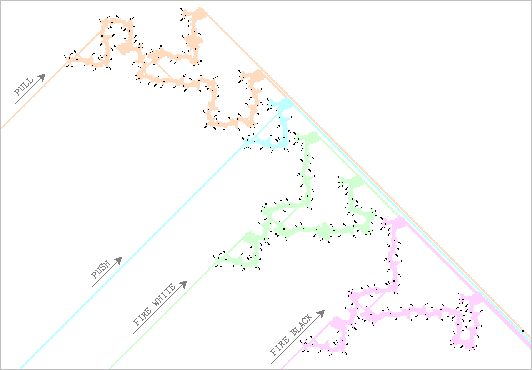
\includegraphics[width=\textwidth]{universal_construction/construction_arm.pdf}}
	\caption{An elbow-operation circuit, which takes a glider on one of four input glider lanes and as a result either pulls or pushes the sliding block (elbow), or uses it to fire a perpendicular glider of either color to the southwest. Note that all four actions require the \texttt{PULL} circuit to be activated, as it produces the frontmost pair of gliders in all four operations (see Exercise~\ref{exer:construction_arm_lanes_timed}). Constructed by Paul Chapman in 2004.}\label{fig:construction_arm}
\end{figure}

By aiming the output gliders of two of these elbow-operation circuits at each other, we can encode the construction of any glider-synthesizable pattern in the input streams (with the advantage that the input lanes are fixed, whereas the output lanes are not).\footnote{This is similar to how we encoded the synthesis of a $2$-engine Cordership in some glider sequences back in Figure~\ref{fig:armless_cordership_gun}.} For example, the pattern displayed in Figure~??...

% FIGURE

% Somewhere: a bit more on its construction itself. Starting top-to bottom, one still life at a time.


%%%%%%%%%%%%%%%%%%%%%%%%%%%%%%%%
\subsection{The Spaceship Itself}\label{sec:gemini_itself}
%%%%%%%%%%%%%%%%%%%%%%%%%%%%%%%%

Importantly, because these circuits are made up of such simple components (mostly blocks and eater~1s, with the most difficult piece to synthesize being a tub), they can even be used to synthesize copies of \emph{themselves}. Indeed, this is the key idea behind the Gemini spaceship: use an extremely long chain of gliders to have two of these circuits build copies of themselves somewhere else in the plane. To turn this idea into a \emph{spaceship} though (rather than just something that repeatedly builds copies of itself), we need to make two additions:\smallskip

\begin{itemize}
	\item[1)] We need to destroy the original pair of elbow-operation circuits after they have constructed the new ones. To do this, we simply use a third elbow-operation circuit, which is constructed alongside the original pair. After all three circuits are constructed, the first two start construction again while the third one starts destroying the old circuits. Since objects like blocks and eater~1s can easily be destroyed by a single glider each, it is straightforward to find a glider recipe that destroys the elbow-operation circuits.\smallskip
	
	\item[2)] We need to be able to re-use the glider recipes that store the construction and destruction recipes. Since we cannot use a static loop (we need the glider recipes to move along with the elbow-operation circuits), we instead have the glider recipes bounce back and forth between \emph{two} copies of the entire three-elbow-operation circuit that we have described.\footnote{In fact, the two ends of the spaceship that we construct will be exactly identical. This is the reason for its name ``Gemini''---it is Latin for ``twins''.}\smallskip
\end{itemize}

After we put all of these ideas together, we get the Gemini spaceship that is displayed in Figure~\ref{fig:gemini}.\footnote{Constructed by Andrew J.~Wade in May 2010.} It builds a copy of itself displaced by 5,120 cells in one direction and 1,024 cells in the other direction every 33,699,586 generations, making it the first spaceship that we have seen that does not travel orthogonally or diagonally at a slope of~$1$ (its slope is $5120/1024 = 5$).

\begin{figure}[!htbp]
	\centering
	\embedlink{gemini}{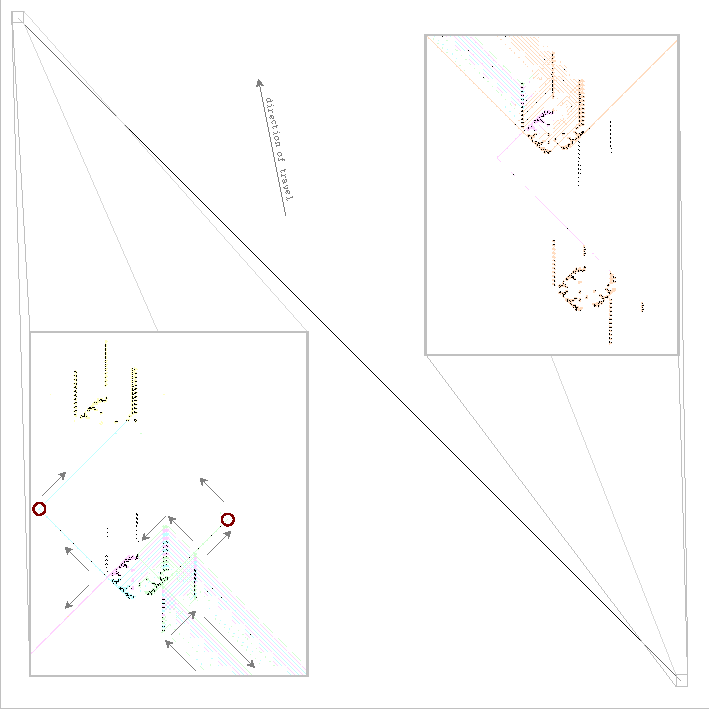
\includegraphics[width=\textwidth]{universal_construction/gemini.pdf}}
	\caption{The self-constructing \emph{Gemini} spaceship, which simply looks like a long, thin diagonal line when zoomed out far enough to see in its entirety. The bulk of the spaceship of made up of 24 parallel glider lanes (12 travelling in each direction), which carry a recipe for building the ship. The ends of the spaceship, which are zoomed in on here, are identical arrangements of stable glider reflectors, glider duplicators, and three elbow-operation circuits whose sliding blocks are circled in \bgbox{redback}{red}. The elbow-operation circuits highlighted in \bgbox{aquaback}{aqua} and \bgbox{greenpastel}{green} build the next copy of the spaceship (highlighted in \bgbox{yellowback2}{yellow}), while the elbow-operation circuit higlighted in \bgbox{magentaback}{magenta} destroys the previous copy of the spaceship (highlighted in \bgbox{orangeback2}{orange}).}\label{fig:gemini}
\end{figure}


%%%%%%%%%%%%%%%%%%%%%%%%%%%%%%%%
\subsection{Geminoids}\label{sec:geminoids}\index{geminoid}
%%%%%%%%%%%%%%%%%%%%%%%%%%%%%%%%

Stuff.
% Describe how fast we can make it go, what the limiting factor is. Say not worth showing variations in bookks since they look essentially identical.



%%%%%%%%%%%%%%%%%%%%%%%%%%%%%%%%
\section{Single-Channel Glider Synthesis with a 90-Degree Elbow}\label{sec:single_channel_synth}\index{elbow}\index{90-degree elbow}
%%%%%%%%%%%%%%%%%%%%%%%%%%%%%%%%

Recall from Section~\ref{sec:slow_salvo} that slow salvo synthesis is a method of encoding the construction of a pattern in the positions of a sequence gliders, with their timing playing no role (except that the gap between consecutive gliders must be sufficiently large that each glider's collision must settle down before the next glider arrives). We now flip this idea around and instead show how to encode the construction of a pattern in the \emph{timing} of a sequence of gliders, with their \emph{position} playing no role. In particular, we show how to encode glider synthesis via gliders that are all coming from the same direction on the same lane.


%%%%%%%%%%%%%%%%%%%%%%%%%%%%%%%%
\subsection{Creating Slow Gliders}\label{sec:single_channel_create_perp_glider}
%%%%%%%%%%%%%%%%%%%%%%%%%%%%%%%%

As with many of our other universal constructions, we make use of a block that acts as an elbow in order to make these single-lane syntheses possible. In particular, we fire a stream of gliders at a block so as to first create a chaotic explosion (but turning the block into a pi-heptomino), and then clean up the resulting debris while creating a perpendicular glider. For example, Figure~\ref{fig:90_degree_first_example} displays a sequence of 13~gliders that, when it collides with a block, produces a single glider travelling in a different direction.

\begin{figure}[!htb]
	\centering
	\patternlink{90_degree_first_example}{\vcenteredhbox{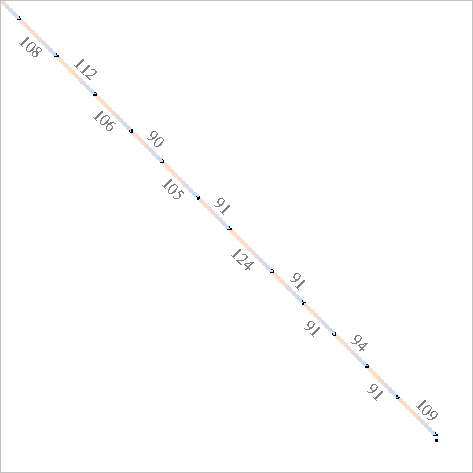
\includegraphics[width=0.486864\textwidth]{universal_construction/90_degree_first_example.pdf}} \vcenteredhbox{\begin{tabular}{@{}c@{}}\color{black}{$\xrightarrow{\text{\clock{3}{3} 1186}}$} \\ \gliderarrow{13}\end{tabular}} \vcenteredhbox{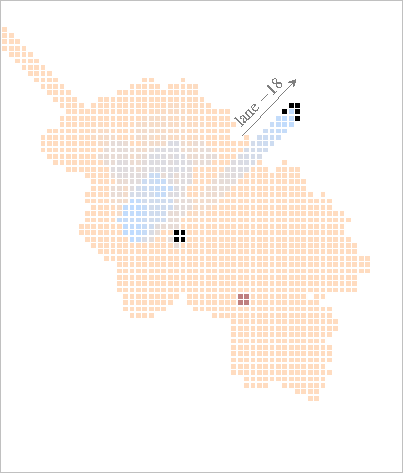
\includegraphics[width=0.414736\textwidth]{universal_construction/90_degree_first_example_2.pdf}}}
	\caption{A sequence of $13$ gliders travelling along the same lane that collide with a block so as to (a) produce a single perpendicular glider, and (b) recreate the target block along the same lane (but shifted northwest by 20 half-diagonals) so that it can be re-used by other single-channel recipes. The numbers on the left indicate the number of generations between consecutive gliders.}\label{fig:90_degree_first_example}
\end{figure}

Since all gliders in a single-channel sequence like this come from the same direction on the same lane, we can encode it simply via the number of generations between each consecutive pair of gliders. For example, the $13$-glider sequence from Figure~\ref{fig:90_degree_first_example} could be encoded by the following sequence of $12$~timing gaps:
\begin{center}
	\texttt{109, 91, 94, 91, 91, 124, 91, 105, 90, 106, 112, 108}.
\end{center}

Computer searches have been carried out\footnote{Mostly by Simon Ekstr{\"o}m, with some optimizations by Dave Greene, in 2017.} to generate single-channel glider sequences that, when aimed at a block as in Figure~\ref{fig:90_degree_first_example} (i.e., so that the first glider triggers a block-to-pi-heptomino explosion), a single output glider is produced on some perpendicular lane. A summary of some reasonably short sequences of this type that produce gliders on a variety of different output lanes (and in either of the two perpendicular output directions) is provided in Table~\ref{tab:single_lane_90deg_glider_timings}.

\newcolumntype{L}{>{\hspace*{-\tabcolsep}}r}
\newcolumntype{R}{l<{\hspace*{-\tabcolsep}}}
\begin{table}[!htb]
	\centering
	\begin{tabular}{@{\hskip 0.31cm}L@{\hskip 0.27cm}r@{\hskip 0.27cm}R@{\hskip 0.34cm}}\toprule
		Lane & Move & Timings \\\midrule
		\texttt{-18i} & \texttt{-20} & \footnotesize\texttt{109,91,94,91,91,124,91,105,90,106,112,108,{\color{gray}(90)}}\\
		\rowcolor{gray!20}\texttt{-15i} & \texttt{-4} & \footnotesize\texttt{109,90,93,91,91,92,90,90,91,90,110,90,90,91,124,133,90,91,113,90,90,{\color{gray}(90)}}\\
		\texttt{-7i} & \texttt{-25} & \footnotesize\texttt{109,91,94,91,91,136,91,90,91,104,90,90,90,110,90,90,98,{\color{gray}(90)}}\\
		\rowcolor{gray!20}\texttt{1i} & \texttt{2} & \footnotesize\texttt{109,91,94,91,90,96,90,91,146,240,109,91,94,91,91,92,90,143,90,91,158,{\color{gray}(90)}}\\
		\texttt{3i} & \texttt{-27} & \footnotesize\texttt{109,90,93,91,91,142,90,109,91,92,90,92,90,118,91,91,90,90,119,{\color{gray}(90)}}\\
		\rowcolor{gray!20}\texttt{5i} & \texttt{8} & \footnotesize\texttt{109,91,94,91,91,136,91,90,91,139,98,90,156,{\color{gray}(133)}}\\
		\texttt{8i} & \texttt{-8} & \footnotesize\texttt{109,90,95,245,90,126,208,128,90,96,91,90,90,91,91,91,91,100,90,90,{\color{gray}(90)}}\\
		\rowcolor{gray!20}\texttt{19i} & \texttt{15} & \footnotesize\texttt{109,91,94,91,91,92,90,97,91,90,91,90,149,90,98,91,90,95,{\color{gray}(90)}}\\\midrule
		\texttt{-21x} & \texttt{-37} & \footnotesize\texttt{109,91,93,90,155,106,90,90,92,91,109,90,93,91,90,100,124,{\color{gray}(90)}}\\
		\rowcolor{gray!20}\texttt{-15x} & \texttt{-26} & \footnotesize\texttt{109,91,93,91,127,91,90,113,90,90,111,90,111,91,91,91,{\color{gray}(90)}}\\
		\texttt{-11x} & \texttt{8} & \footnotesize\texttt{109,91,94,91,91,136,91,90,91,101,90,90,90,92,90,144,90,91,90,90,126,{\color{gray}(90)}}\\
		\rowcolor{gray!20}\texttt{-9x} & \texttt{16} & \footnotesize\texttt{109,91,94,91,91,136,91,90,91,168,90,90,97,91,91,91,90,116,90,90,90,90,90,{\color{gray}(90)}}\\
		\texttt{-3x} & \texttt{-15} & \footnotesize\texttt{109,91,93,91,97,91,91,106,91,90,90,90,90,90,91,163,90,90,104,{\color{gray}(90)}}\\
		\rowcolor{gray!20}\texttt{-1x} & \texttt{-5} & \footnotesize\texttt{109,91,94,91,91,136,91,90,91,139,98,90,94,90,95,90,91,118,207,93,{\color{gray}(90)}}\\
		\texttt{2x} & \texttt{3} & \footnotesize\texttt{109,91,94,91,91,92,90,143,90,91,158,{\color{gray}(90)}}\\
		\rowcolor{gray!20}\texttt{10x} & \texttt{11} & \footnotesize\texttt{109,91,94,91,91,92,90,119,90,90,109,91,94,91,91,92,90,143,90,91,158,{\color{gray}(90)}}\\
		\bottomrule
	\end{tabular}
	\caption{Single-channel glider sequences that collide with a 90-degree elbow so as to produce a perpendicular output glider on a given lane. The first 8 rows give sequences that produce an ``\textbf{i}nternal'' glider (i.e., one that travels northeast when oriented as in Figure~\ref{fig:90_degree_first_example}) and the last 8 rows give sequences that produce an ``e\textbf{x}ternal'' glider (i.e., one that travels southwest). The ``move'' column indicates how many half-diagonals the elbow is moved forward or backward, and the ``timings'' column indicates the number of generations between consecutive gliders in the sequence. The final number in parentheses is the number of generations that must pass before it is safe to send subsequent glider sequences.}\label{tab:single_lane_90deg_glider_timings}
\end{table}

There are numerous points of clarification that we need to make about these sequences:\smallskip

\begin{itemize}
	\item The output lane number has either an ``\texttt{i}'' or ``\texttt{x}'' suffix, indicating in which of the two perpendicular directions the output glider travels. The suffixes stand for \textbf{i}nternal and e\textbf{x}ternal, which refer to the output glider travelling on the same side as the elbow block that the input glider sequence hits, or the opposite side, respectively.\smallskip 
	
	\item Some of these glider sequences, like the one with output on lane~2x, change the zero-degree elbow block into another small object like a boat, beehive, or pond. This is okay because those objects explode into a pi-heptomino when they are hit by a glider in the exact same way that a block does, and this is always the reaction that the first glider in these single-channel sequence triggers.\smallskip
	
	\item The ``move'' column of Table~\ref{tab:single_lane_90deg_glider_timings} specifies how many half-diagonals farther away the zero-degree elbow is moved by the glider sequence.\smallskip
	
	\item The value in the ``move'' column being odd means that the elbow was moved to the other side of the input glider stream. If this happens, the output lanes of all subsequent glider sequences are flipped from \texttt{i} to \texttt{x}, and vice-versa. For example, the sequence corresponding to lane~$2x$ has a ``move'' value of $3$, which is odd. Thus if we want to output gliders on lanes $2x$ and then $-12x$, we would have to send the sequences corresponding to lanes $2x$ and then $-15i$ (not $-15x$).\smallskip
	
	\item In most of these glider sequences, there are numerous gaps of 90 and 91~generations. The reason for this is that we want to be able to feed these single-channel glider recipes through standard components like Snarks and the easy-to-synthesize Lx200-assisted\index{Lx200} syringe\index{syringe} from Exercise~\ref{exer:syringe_Lx200} (which has a repeat time of~$90$ generations).\footnote{Single-channel glider sequences with large timing gaps are desirable since they can make use of circuitry that has a higher repeat time. We could use sequences with gaps no smaller than $153$~generations (such sequences are known to be able to emulate arbitrary glider syntheses), thus letting us feed these sequences through the syringe variant from Figure~\ref{fig:syringe_modified}, for example. However, as the minimum timing gap increases, so does the length of the resulting glider sequences, so we stick with a minimum timing gap of 90~generations.}
	
	Most of the gliders that have a timing of 90 or 91 generations could actually be moved much closer (i.e., the previous glider's collision settles down before they arrive) if we so desired. The reason that some gliders use a gap of $91$~generations instead of just $90$ is that their timing matters mod~$2$, due to p$2$ components like blinkers in an intermediate reaction.\smallskip
\end{itemize}


%%%%%%%%%%%%%%%%%%%%%%%%%%%%%%%%
\subsection{Moving the Elbow}\label{sec:single_channel_move_elbow}
%%%%%%%%%%%%%%%%%%%%%%%%%%%%%%%%

The sequences given in Table~\ref{tab:single_lane_90deg_glider_timings} can only be used to fire gliders on a small selection of lanes (8 in each direction). Furthermore, these sequences move the elbow forward and backward by some amount that we do not control---an amount that is dictated by the output lane on which we wish to fire a glider. It is thus important to be able to move the elbow however far forward or backward we like, \emph{without} firing a glider, so that the glider-firing sequences then produce a glider where we actually want it. For example, the following pair of elbow-moving sequences, which are displayed in Figure~\ref{fig:0_degree_block_push_pull}, move the elbow forward by $8$~half diagonals or backward by $12$ half diagonals, respectively.
\begin{align*}
	& \text{\texttt{~push~8hd: \footnotesize 109, 91, 94, 91, 91, 92, 90, 119, 90, {\color{gray}(90)},}}\\
	& \text{\texttt{pull~12hd: \footnotesize 109, 91, 93, 91, 137, 91, 91, 125, 172, 108, 90, 109, 91, 101, 120, 90, {\color{gray}(90)}.}}
\end{align*}

\begin{figure}[!htb]
	\centering
	\begin{tabular}{@{}cc@{}}
		\begin{subfigure}{0.48\textwidth}
			\centering
			\patternlink{0_degree_block_push}{\vcenteredhbox{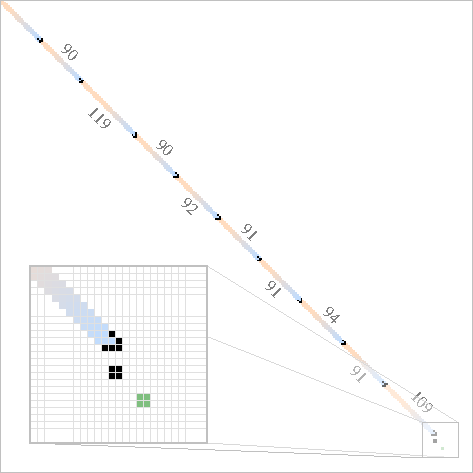
\includegraphics[width=\textwidth]{universal_construction/0_degree_block_push.pdf}}}
			\caption{push 8 half diagonals}
			\label{fig:0_degree_block_push}
		\end{subfigure} & \begin{subfigure}{0.48\textwidth}
			\centering
			\patternlink{0_degree_block_pull}{\vcenteredhbox{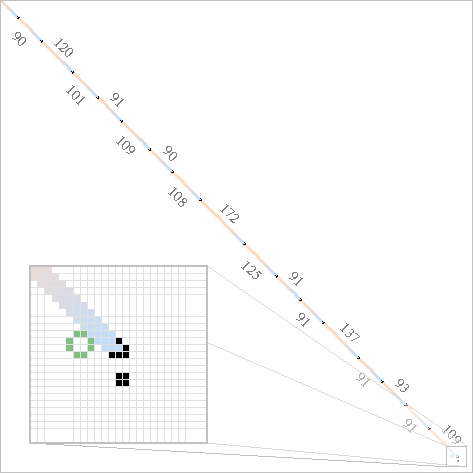
\includegraphics[width=\textwidth]{universal_construction/0_degree_block_pull.pdf}}}
			\caption{pull 12 half diagonals}
			\label{fig:0_degree_block_pull}
		\end{subfigure}
	\end{tabular}
	\caption{Single-channel glider sequences that (a) push or (b) pull an elbow. The location of the elbow after being pushed or pulled is marked in \bgbox{greenpastel}{green}.}\label{fig:0_degree_block_push_pull}
\end{figure}

A more complete summary of elbow-moving sequences is given in Table~\ref{tab:single_lane_elbow_movers}, which tells us how to move the $90$-degree elbow in either direction by any number of half-diagonals up to $10$. To move the elbow by a larger amount, we can simply repeat these sequences.

\begin{table}[!htb]
	\centering
	\begin{tabular}{@{\hskip 0.31cm}L@{\hskip 0.27cm}R@{\hskip 0.34cm}}\toprule
		Move & Timings \\\midrule
		\texttt{-10} & \footnotesize\texttt{109,91,94,91,91,96,90,97,91,91,130,94,90,105,90,95,111,{\color{gray}(90)}}\\
		\rowcolor{gray!20} \texttt{-9} & \footnotesize\texttt{109,91,94,91,91,179,90,91,94,91,102,91,105,91,108,90,91,91,120,90,{\color{gray}(90)}}\\
		\texttt{-8} & \footnotesize\texttt{109,90,93,91,90,95,91,90,91,91,90,90,91,90,90,99,90,90,91,90,94,90,{\color{gray}(90)}}\\
		\rowcolor{gray!20} \texttt{-7} & \footnotesize\texttt{109,91,93,91,118,90,91,91,91,90,90,156,114,90,90,90,90,141,{\color{gray}(90)}}\\
		\texttt{-6} & \footnotesize\texttt{109,91,93,91,156,91,91,94,90,91,140,91,103,91,91,132,{\color{gray}(90)}}\\
		\rowcolor{gray!20} \texttt{-5} & \footnotesize\texttt{109,91,94,91,91,92,90,173,100,90,141,91,90,90,90,147,90,117,{\color{gray}(192)}}\\
		\texttt{-4} & \footnotesize\texttt{109,90,93,91,91,90,90,92,90,95,91,170,90,90,91,91,98,91,91,{\color{gray}(90)}}\\
		\rowcolor{gray!20} \texttt{-3} & \footnotesize\texttt{109,91,94,91,90,96,90,91,92,90,217,90,103,{\color{gray}(90)}}\\
		\texttt{-2} & \footnotesize\texttt{109,91,94,91,91,136,90,90,91,171,100,118,90,{\color{gray}(90)}}\\
		\rowcolor{gray!20} \texttt{-1} & \footnotesize\texttt{109,91,94,91,90,96,90,91,146,{\color{gray}(240)}}\\\midrule
		\texttt{1} & \footnotesize\texttt{109,91,94,91,91,92,90,143,90,91,156,90,104,{\color{gray}(164)}}\\
		\rowcolor{gray!20} \texttt{2} & \footnotesize\texttt{109,90,93,91,91,90,90,91,91,90,90,91,90,90,94,90,{\color{gray}(90)}}\\
		\texttt{3} & \footnotesize\texttt{109,91,94,91,91,92,90,143,90,90,90,129,101,102,{\color{gray}(90)}}\\
		\rowcolor{gray!20} \texttt{4} & \footnotesize\texttt{109,91,93,91,92,90,90,90,151,93,90,143,134,94,90,90,90,109,91,{\color{gray}(90)}}\\
		\texttt{5} & \footnotesize\texttt{109,91,93,91,92,90,110,90,152,90,90,91,91,91,90,90,90,90,175,119,115,{\color{gray}(193)}}\\
		\rowcolor{gray!20} \texttt{6} & \footnotesize\texttt{109,91,93,91,145,215,104,90,90,90,90,90,102,92,90,90,90,106,155,150,{\color{gray}(90)}}\\
		\texttt{7} & \footnotesize\texttt{109,91,94,91,90,96,90,91,146,240,109,91,94,91,91,92,90,119,90,{\color{gray}(90)}}\\
		\rowcolor{gray!20} \texttt{8} & \footnotesize\texttt{109,91,94,91,91,92,90,119,90,{\color{gray}(90)}}\\
		\texttt{9} & \footnotesize\texttt{109,90,93,91,91,90,90,95,90,91,90,90,140,90,90,128,{\color{gray}(93)}}\\
		\rowcolor{gray!20} \texttt{10} & \footnotesize\texttt{109,91,93,91,129,149,91,90,90,105,90,90,90,90,114,91,100,90,{\color{gray}(90)}}\\\bottomrule
	\end{tabular}
	\caption{Single-channel glider sequences that can be used to move the 90-degree elbow to any location along the input glider lane. The ``move'' and ``timings'' columns are as in Table~\ref{tab:single_lane_90deg_glider_timings}.}\label{tab:single_lane_elbow_movers}
\end{table}

With these block-moving sequences at our disposal, we are now able to use gliders on a single lane to fire slow perpendicular gliders on any sequence of lanes of our choosing: by repeating the sequences from Table~\ref{tab:single_lane_elbow_movers} we can move the elbow to any lane that we like, and we can then use a sequence from Table~\ref{tab:single_lane_90deg_glider_timings} to  actually fire a perpendicular glider.


%%%%%%%%%%%%%%%%%%%%%%%%%%%%%%%%
\subsection{Creating and Using a Hand}\label{sec:single_channel_hand}
%%%%%%%%%%%%%%%%%%%%%%%%%%%%%%%%

The only extra ingredient that we need in order to show that single-channel glider synthesis with a 90-degree elbow block is universal (i.e., can implement any glider synthesis) is a way of creating a target block (which we refer to as a \emph{hand}\footnote{It is connected to an elbow, after all.})\index{hand} that the perpendicular slow gliders will be fired at. One sequence of gliders that works to create such a hand block is
\begin{align}\begin{split}\label{eq:make_hand_90_deg}
	& \text{\texttt{109, 91, 93, 90, 132, 115, 127, 91, 90, 91, 95, 90, 114,}} \\
	& \text{\texttt{~~~~~~~~~162, 233, 159, 90, 155, 126, 93, 118, 90, 91, 90, {\color{gray}(90)},}}
\end{split}\end{align}
which is illustrated as the first transition in Figure~\ref{fig:90_degree_block_move}. Indeed, this recipe creates a hand block $86$ half-diagonals away, on the internal side of the elbow block, while pushing that elbow block away by $17$ half~diagonals.\footnote{In particular, since we have described the elbow block as moving by an odd number of half-diagonals, we know that it moves to the opposite side of the single-lane glider sequence.}

Since we can now use single-channel glider sequences and a $90$-degree elbow to create slow gliders on any lane, and we can also create a hand block for those gliders to collide with, we immediately see from Theorem~\ref{thm:p1_slow_salvo} that these types of glider syntheses are universal. That is, we have demonstrated the following result:

\begin{theorem}\label{thm:single_channel_90_degree}
	Every pattern that can be constructed via glider synthesis can be constructed by a single-channel glider synthesis with a $90$-degree elbow.
\end{theorem}

To illustrate how to implement slow salvo synthesis via single-channel synthesis, consider the problem of moving the hand block after we create it. We can use any of the slow salvos from Figures~\ref{fig:block_movers} and~\ref{fig:p2_block_movers} to carry out this task---we will implement the $4$-glider $(11,0)$ block pull\index{(11,0) block pull} from Figure~\ref{fig:block_move_11_0}, which uses gliders on lanes (relative to the initial position of the elbow block) $-6i$, $-6i$, $6i$, and $0i$, in that order.

To this end, we first use the hand-making sequence of gliders~\eqref{eq:make_hand_90_deg}, which moves the block to position~$17$. We can then fire the four slow gliders as follows:\smallskip

\begin{itemize}
	\item We want to fire a glider $17 - (-6) = 23$ lanes behind the elbow. Since the hand-making sequence of gliders flipped the orientation of the elbow block, we thus want to fire the first glider on lane $-23x$ (not $-23i$). This can be achieved by a $-2$ half-diagonal elbow move (from Table~\ref{tab:single_lane_elbow_movers}) followed by firing a glider on lane $-21x$ (from Table~\ref{tab:single_lane_90deg_glider_timings}).\smallskip
	
	\item Since firing a glider on lane $-21x$ moved the elbow by $-37$ half-diagonals (which is odd, so the elbow's orientation is flipped back to where it started), the elbow is now on lane $17 - 2 - 37 = -22$. We want to fire a glider $-22 - (-6) = -16$ lanes behind the elbow, which is lane $16i$. This can be achieved by pushing the elbow forward by $8$hd and then firing on lane $8i$.\smallskip
	
	\item Since firing on lane $8i$ moved the elbow by $-8$hd, it is now on lane $-22 + 8 - 8 = -22$. We want to fire a glider $-22 - 6 = -28$ lanes behind the elbow, which is lane $28i$. This can be achieved by pushing the elbow forward by $10$hd, pushing it by $10$hd again, and then firing on lane $8i$.\footnote{Be careful---we cannot just push the elbow forward by $9$hd and then fire on lane $19i$, since the $9$hd move would flip the orientation of the block, meaning you would have to fire on lane $19x$ instead.}\smallskip
	
	\item Finally, since firing on lane $8i$ moved the elbow backward by $8$hd, it is now on lane $-22 + 10 + 10 - 8 = -10$. We want to fire a glider $-10 - 0 = -10$ lanes behind the elbow, which is lane $10i$. This can be achieved by a $2$hd elbow move followed by firing a glider on lane $8i$.\smallskip
\end{itemize}

When we put all of this together, we get the following single-lane sequence of 185 gliders (which we illustrate in Figure~\ref{fig:90_degree_block_move} and specify by 184 timings between those gliders) that first creates a hand block and then moves that hand block $11$~cells via a sequence of $4$ perpendicular slow gliders:\footnote{We did something slightly tricky with with the two ``move 10hd'' sequences here---notice that the gap between their final pair of gliders are not the same as each other. See Exercise~\ref{exer:single_lane_glider_final_glider_explain}.}
\begin{align*}
		& \text{\texttt{\footnotesize make hand: {\scriptsize 109, 91, 93, 90, 132, 115, 127, 91, 90, 91, 95, 90, 114, 162, 233, 159, 90, 155, 126, 93,}}} \\
		& \text{\texttt{\footnotesize ~~~~~~~~~~~~{\scriptsize 118, 90, 91, 90, 90,}}} \\
		& \text{\texttt{\footnotesize move -2hd: {\scriptsize 109, 91, 94, 91, 91, 136, 90, 90, 91, 171, 100, 118, 90, 90,}}} \\
		& \text{\texttt{\footnotesize fire -21x: {\scriptsize 109, 91, 93, 90, 155, 106, 90, 90, 92, 91, 109, 90, 93, 91, 90, 100, 124, 90,}}} \\
		& \text{\texttt{\footnotesize move~~8hd: {\scriptsize 109, 91, 94, 91, 91, 92, 90, 119, 90, 90,}}} \\
		& \text{\texttt{\footnotesize fire~~~8i: {\scriptsize 109, 90, 95, 245, 90, 126, 208, 128, 90, 96, 91, 90, 90, 91, 91, 91, 91, 100, 90, 90, 90,}}} \\
		& \text{\texttt{\footnotesize move~10hd: {\scriptsize 109, 91, 93, 91, 129, 149, 91, 90, 90, 105, 90, 90, 90, 90, 114, 91, 100, 90, 90,}}} \\
		& \text{\texttt{\footnotesize move~10hd: {\scriptsize 109, 91, 93, 91, 129, 149, 91, 90, 90, 105, 90, 90, 90, 90, 114, 91, 100, 90, 91,}}} \\
		& \text{\texttt{\footnotesize fire~~~8i: {\scriptsize 109, 90, 95, 245, 90, 126, 208, 128, 90, 96, 91, 90, 90, 91, 91, 91, 91, 100, 90, 90, 90,}}} \\
		& \text{\texttt{\footnotesize move~~2hd: {\scriptsize 109, 90, 93, 91, 91, 90, 90, 91, 91, 90, 90, 91, 90, 90, 94, 90, 90,}}} \\
		& \text{\texttt{\footnotesize fire~~~8i: {\scriptsize 109, 90, 95, 245, 90, 126, 208, 128, 90, 96, 91, 90, 90, 91, 91, 91, 91, 100, 90, 90.}}}
\end{align*}

\begin{figure}[!htb]
	\centering
	\embedlink{90_degree_block_move}{\vcenteredhbox{\phantom{$\cdots$ $\xrightarrow{\text{\clock{2}{12} 1720}}$}} \vcenteredhbox{\patternimg{0.07}{90_degree_block_move_0}} \vcenteredhbox{\begin{tabular}{@{}c@{}}\color{black}{$\xrightarrow{\text{\clock{7}{1} 2859}}$} \\ \gliderarrow{25}\end{tabular}} \vcenteredhbox{\patternimg{0.07}{90_degree_block_move_1}} \vcenteredhbox{\begin{tabular}{@{}c@{}}\color{black}{$\xrightarrow{\text{\clock{11}{20} 1448}}$} \\ \gliderarrow{14}\end{tabular}} \vcenteredhbox{\patternimg{0.07}{90_degree_block_move_2}}} \\[1em]
	
	\patternlink{90_degree_block_move}{\vcenteredhbox{\begin{tabular}{@{}c@{}}\color{black}{$\cdots$ $\xrightarrow{\text{\clock{2}{12} 1720}}$} \\ \hphantom{$\cdots$} \gliderarrow{18}\end{tabular}} \vcenteredhbox{\patternimg{0.07}{90_degree_block_move_3}} \vcenteredhbox{\begin{tabular}{@{\hskip 0.09cm}c@{\hskip 0.09cm}}\color{black}{$\xrightarrow{\text{\clock{1}{52} 973}}$} \\ \gliderarrow{10}\end{tabular}} \vcenteredhbox{\patternimg{0.07}{90_degree_block_move_4}} \vcenteredhbox{\begin{tabular}{@{}c@{}}\color{black}{$\xrightarrow{\text{\clock{9}{25} 2266}}$} \\ \gliderarrow{21}\end{tabular}} \vcenteredhbox{\patternimg{0.07}{90_degree_block_move_5}}} \\[1em]
	
	\patternlink{90_degree_block_move}{\vcenteredhbox{\begin{tabular}{@{}c@{}}\color{black}{$\cdots$ $\xrightarrow{\text{\clock{2}{12} 1903}}$} \\ \hphantom{$\cdots$} \gliderarrow{19}\end{tabular}} \vcenteredhbox{\patternimg{0.07}{90_degree_block_move_6}} \vcenteredhbox{\begin{tabular}{@{}c@{}}\color{black}{$\xrightarrow{\text{\clock{2}{13} 1904}}$} \\ \gliderarrow{19}\end{tabular}} \vcenteredhbox{\patternimg{0.07}{90_degree_block_move_7}} \vcenteredhbox{\begin{tabular}{@{}c@{}}\color{black}{$\xrightarrow{\text{\clock{9}{25} 2266}}$} \\ \gliderarrow{21}\end{tabular}} \vcenteredhbox{\patternimg{0.07}{90_degree_block_move_8}}} \\[1em]
	
	\patternlink{90_degree_block_move}{\vcenteredhbox{\begin{tabular}{@{}c@{}}\color{black}{$\cdots$ $\xrightarrow{\text{\clock{8}{5} 1565}}$} \\ \hphantom{$\cdots$} \gliderarrow{17}\end{tabular}} \vcenteredhbox{\patternimg{0.07}{90_degree_block_move_9}} \vcenteredhbox{\begin{tabular}{@{}c@{}}\color{black}{$\xrightarrow{\text{\clock{9}{25} 2266}}$} \\ \gliderarrow{21}\end{tabular}} \vcenteredhbox{\patternimg{0.07}{90_degree_block_move_10}} \vcenteredhbox{\color{black}{\hspace{0.08cm}$\xrightarrow{\text{\clock{6}{45} 138}}$\hspace{0.08cm}}} \vcenteredhbox{\patternimg{0.07}{90_degree_block_move_11}}}
	
	\caption{A single-lane sequence of 185 gliders creating a hand block and then firing 4 perpendicular slow gliders at that hand block so as to move it down by 11~cells. The perpendicular slow gliders are created on the correct lanes by repeatedly adjusting the position of the 90-degree elbow.}\label{fig:90_degree_block_move}
\end{figure}



%%%%%%%%%%%%%%%%%%%%%%%%%%%%%%%%
\section{Single-Channel Glider Synthesis with a Zero-Degree Elbow}\label{sec:single_channel_synth_0}\index{zero-degree elbow}
%%%%%%%%%%%%%%%%%%%%%%%%%%%%%%%%

While the single-channel syntheses of the previous subsection are very useful, it is sometimes desirable to use single-channel glider sequences to build an object directly in front of them, rather than off to their side. For example, it will be useful for us to be able to use gliders from a single lane to construct a Snark that accepts gliders on that same lane as input. To make this possible, instead of using a 90-degree elbow we use a \emph{zero-degree elbow}:\index{zero-degree elbow} a small stable object (like a block) that several gliders are fired at on a particular lane so as to produce a single glider going in the \emph{same direction} but on a different lane.\footnote{Here, ``zero-degree'' refers to the fact that the input glider stream is being ``reflected'' by zero degrees (i.e., not reflected at all, but just shifted to a different lane).}


%%%%%%%%%%%%%%%%%%%%%%%%%%%%%%%%
\subsection{Creating Slow Gliders}\label{sec:single_channel_zero_make_slow}
%%%%%%%%%%%%%%%%%%%%%%%%%%%%%%%%

To illustrate how a zero-degree elbow works, consider the sequence of $14$~gliders displayed in Figure~\ref{fig:lane_8_0degree} that, when it collides with a block, produces a single glider going in the same direction, but shifted by $8$ lanes.

\begin{figure}[!htb]
	\centering
	\patternlink{lane_8_0degree}{\vcenteredhbox{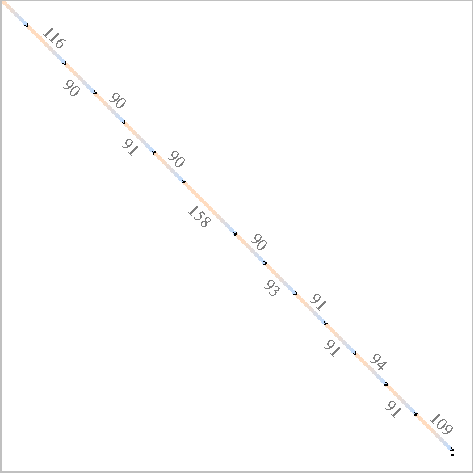
\includegraphics[width=0.4508\textwidth]{universal_construction/lane_8_0degree.pdf}}  \vcenteredhbox{\begin{tabular}{@{}c@{}}\color{black}{$\xrightarrow{\text{\clock{3}{3} 1440}}$} \\ \gliderarrow{14}\end{tabular}} \vcenteredhbox{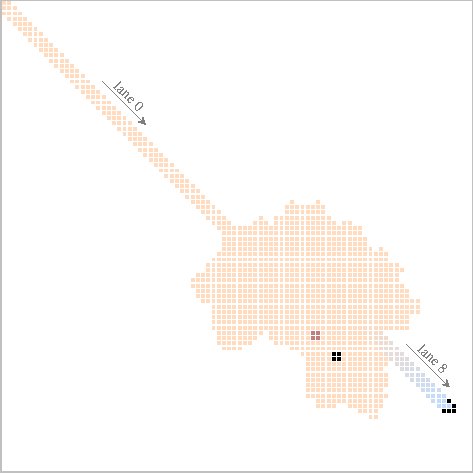
\includegraphics[width=0.4508\textwidth]{universal_construction/lane_8_0degree_2.pdf}}}
	\caption{A sequence of $14$ gliders travelling along the same lane that collide with a block so as to (a) produce a single glider travelling in the same direction, but shifted up by $8$~lanes, and (b) recreate the target block along the same lane (but shifted southeast by 8 half-diagonals) so that it can be re-used by other single-channel recipes.}\label{fig:lane_8_0degree}
\end{figure}

As with $90$-degree single-channel sequences, we encode zero-degree single-channel sequences simply by the number of generations between each consecutive pair of gliders. For example, we encode the $14$-glider sequence from Figure~\ref{fig:lane_8_0degree} via the following sequence of $13$~timing gaps:
\begin{center}
	\texttt{109, 91, 94, 91, 91, 93, 90, 158, 90, 91, 90, 90, 116, {\color{gray}(104)}},
\end{center}
with the final number in gray indicating how many generations must pass before another glider sequence can safely arrive.

In this zero-degree setting, it is much more important to be able to fire output gliders on a wide variety of different lanes than it was in the 90-degree setting. Indeed, when we worked with a 90-degree elbow we were able to simply move the elbow forward or backward to reach different output lanes, but doing so has no effect whatsoever on the output lane in the zero-degree setting.

For this reason, extensive computer searches have been used to generate single-channel glider sequences of this type that produce a single output glider on any lane from $-100$ to $+100$.\footnote{A complete collection of tens of thousands of these recipes can be downloaded from \httpsurl{gitlab.com/apgoucher/slmake/-/tree/master/data/simeks}. It can be useful to have multiple recipes for the same output lane, since they might move the zero-degree elbow by different amounts.} A summary of sequences of this type for output lanes $-22$ through $+22$ is provided in Table~\ref{tab:single_lane_0deg_glider_timings}.

\begin{table}[!phtb]
	\centering
	\begin{tabular}{@{\hskip 0.31cm}L@{\hskip 0.27cm}r@{\hskip 0.27cm}R@{\hskip 0.34cm}}\toprule
		Lane & Move & Timings \\\midrule
		\texttt{-22} & \texttt{-20} & \footnotesize\texttt{109,91,94,91,91,136,90,90,91,114,90,91,90,99,90,97,90,90,90,126,90,137,90,{\color{gray}(90)}} \\
		\rowcolor{gray!20}\texttt{-21} & \texttt{8} & \footnotesize\texttt{109,91,94,91,91,95,91,90,146,91,99,90,118,120,135,90,90,121,{\color{gray}(90)}} \\
		\texttt{-20} & \texttt{-29} & \footnotesize\texttt{93,90,91,91,90,90,91,90,103,113,91,103,90,152,181,140,91,90,166,91,{\color{gray}(106)}} \\
		\rowcolor{gray!20}\texttt{-19} & \texttt{-20} & \footnotesize\texttt{109,91,93,91,171,91,90,90,94,91,106,91,91,90,90,143,90,91,91,91,90,91,112,{\color{gray}(90)}} \\
		\texttt{-18} & \texttt{8} & \footnotesize\texttt{109,90,93,91,91,128,91,91,90,97,90,99,90,139,91,91,117,134,92,90,90,90,{\color{gray}(90)}} \\
		\rowcolor{gray!20}\texttt{-17} & \texttt{-22} & \footnotesize\texttt{109,91,93,91,123,90,129,90,90,111,142,91,90,120,91,142,{\color{gray}(98)}} \\
		\texttt{-16} & \texttt{8} & \footnotesize\texttt{109,91,94,91,91,124,91,126,91,140,162,148,90,90,119,90,{\color{gray}(90)}} \\
		\rowcolor{gray!20}\texttt{-15} & \texttt{13} & \footnotesize\texttt{109,91,93,90,156,91,91,94,91,90,147,117,91,144,90,91,128,100,91,90,105,91,{\color{gray}(90)}} \\
		\texttt{-14} & \texttt{-39} & \footnotesize\texttt{109,91,93,91,155,106,91,91,96,90,90,91,108,90,156,90,90,120,90,112,91,99,{\color{gray}(90)}} \\
		\rowcolor{gray!20}\texttt{-13} & \texttt{1} & \footnotesize\texttt{109,91,93,91,92,90,158,90,94,270,172,130,90,91,91,96,90,90,147,{\color{gray}(90)}} \\
		\texttt{-12} & \texttt{-23} & \footnotesize\texttt{109,91,94,91,90,162,122,111,90,90,90,96,91,91,91,122,91,91,171,{\color{gray}(90)}} \\
		\rowcolor{gray!20}\texttt{-11} & \texttt{-53} & \footnotesize\texttt{93,91,151,90,139,180,103,115,167,91,120,139,135,91,91,{\color{gray}(169)}} \\
		\texttt{-10} & \texttt{15} & \footnotesize\texttt{109,91,93,91,97,91,90,91,120,90,95,91,143,90,90,90,90,{\color{gray}(90)}} \\
		\rowcolor{gray!20}\texttt{-9} & \texttt{-15} & \footnotesize\texttt{109,91,94,91,91,90,91,91,90,158,90,91,90,90,101,90,107,90,90,90,{\color{gray}(90)}} \\
		\texttt{-8} & \texttt{1} & \footnotesize\texttt{93,91,116,90,106,91,143,91,109,90,91,103,110,91,136,91,92,91,155,{\color{gray}(199)}} \\
		\rowcolor{gray!20}\texttt{-7} & \texttt{-34} & \footnotesize\texttt{109,91,93,91,92,91,98,201,91,129,90,90,90,90,90,103,90,108,90,104,{\color{gray}(90)}} \\
		\texttt{-6} & \texttt{-11} & \footnotesize\texttt{109,91,94,91,90,90,90,90,109,91,101,90,98,90,{\color{gray}(90)}} \\
		\rowcolor{gray!20}\texttt{-5} & \texttt{-20} & \footnotesize\texttt{109,91,94,91,91,95,91,90,104,90,90,97,91,91,94,191,97,90,126,{\color{gray}(90)}} \\
		\texttt{-4} & \texttt{-23} & \footnotesize\texttt{0,93,91,90,144,90,111,91,92,91,103,91,144,90,168,91,91,102,90,92,90,94,{\color{gray}(90)}} \\
		\rowcolor{gray!20}\texttt{-3} & \texttt{-9} & \footnotesize\texttt{109,91,94,91,91,136,90,90,91,168,90,106,90,90,138,90,90,106,{\color{gray}(90)}} \\
		\texttt{-2} & \texttt{7} & \footnotesize\texttt{109,91,93,91,92,91,90,90,162,91,91,90,129,91,113,90,90,90,{\color{gray}(90)}} \\
		\rowcolor{gray!20}\texttt{-1} & \texttt{-9} & \footnotesize\texttt{109,90,95,245,90,95,90,123,91,90,115,142,{\color{gray}(90)}} \\\midrule
		\texttt{0} & \texttt{-1} & \scriptsize\texttt{109,91,93,91,92,90,97,91,116,91,145,90,91,98,90,90,188,91,90,90,{\color{gray}(90)}} \\\midrule
		\rowcolor{gray!20}\texttt{1} & \texttt{-24} & \scriptsize\texttt{109,91,94,91,91,93,90,95,90,113,90,99,90,156,90,90,90,138,{\color{gray}(170)}} \\
		\texttt{2} & \texttt{-27} & \scriptsize\texttt{109,91,94,91,91,124,91,90,91,91,90,91,90,141,90,172,91,161,90,169,228,{\color{gray}(90)}} \\
		\rowcolor{gray!20}\texttt{3} & \texttt{4} & \scriptsize\texttt{109,91,94,91,91,92,90,169,90,90,90,107,90,90,91,90,95,91,{\color{gray}(90)}} \\
		\texttt{4} & \texttt{-56} & \scriptsize\texttt{109,91,94,91,91,92,90,169,91,90,116,90,161,91,104,{\color{gray}(90)}} \\
		\rowcolor{gray!20}\texttt{5} & \texttt{-8} & \footnotesize\texttt{109,90,93,91,91,135,91,124,90,90,148,91,91,97,141,91,{\color{gray}(90)}} \\
		\texttt{6} & \texttt{-15} & \scriptsize\texttt{93,90,90,90,91,90,91,136,155,98,120,90,90,91,92,90,97,161,161,{\color{gray}(139)}} \\
		\rowcolor{gray!20}\texttt{7} & \texttt{-30} & \footnotesize\texttt{109,91,94,91,91,124,91,105,90,169,91,90,116,91,142,90,90,{\color{gray}(90)}} \\
		\texttt{8} & \texttt{8} & \scriptsize\texttt{109,91,94,91,91,93,90,158,90,91,90,90,116,{\color{gray}(104)}} \\
		\rowcolor{gray!20}\texttt{9} & \texttt{11} & \footnotesize\texttt{109,91,93,90,171,90,90,91,90,91,90,91,129,144,90,90,120,90,91,91,169,90,{\color{gray}(90)}} \\
		\texttt{10} & \texttt{14} & \scriptsize\texttt{109,91,93,90,140,150,108,91,90,111,91,91,194,98,90,169,{\color{gray}(90)}} \\
		\rowcolor{gray!20}\texttt{11} & \texttt{-5} & \scriptsize\texttt{109,91,94,91,91,92,90,146,90,90,90,91,135,91,152,{\color{gray}(135)}} \\
		\texttt{12} & \texttt{8} & \scriptsize\texttt{91,94,91,91,121,90,90,90,90,90,90,99,90,165,119,90,106,90,90,{\color{gray}(90)}} \\
		\rowcolor{gray!20}\texttt{13} & \texttt{-32} & \scriptsize\texttt{109,91,94,91,91,96,90,97,91,91,145,90,113,90,90,105,91,193,{\color{gray}(90)}} \\
		\texttt{14} & \texttt{-16} & \scriptsize\texttt{109,91,93,91,129,149,91,90,90,142,219,90,99,91,109,115,92,185,{\color{gray}(90)}} \\
		\rowcolor{gray!20}\texttt{15} & \texttt{9} & \scriptsize\texttt{109,90,93,91,91,158,94,113,91,90,91,96,90,142,{\color{gray}(90)}} \\
		\texttt{16} & \texttt{8} & \scriptsize\texttt{109,91,94,91,91,95,91,90,93,218,172,90,90,90,116,112,341,107,106,90,163,91,{\color{gray}(90)}} \\
		\rowcolor{gray!20}\texttt{17} & \texttt{-28} & \scriptsize\texttt{109,91,94,91,91,96,90,166,91,91,114,90,90,91,90,90,114,91,101,{\color{gray}(90)}} \\
		\texttt{18} & \texttt{1} & \scriptsize\texttt{109,90,93,91,91,148,91,90,151,90,91,163,108,151,112,144,90,149,90,90,99,{\color{gray}(90)}} \\
		\rowcolor{gray!20}\texttt{19} & \texttt{-19} & \scriptsize\texttt{109,91,93,91,115,107,90,90,90,90,90,90,90,103,99,118,91,130,{\color{gray}(90)}} \\
		\texttt{20} & \texttt{12} & \scriptsize\texttt{109,91,93,90,169,90,91,103,91,133,90,90,91,91,90,110,91,93,90,112,171,{\color{gray}(90)}} \\
		\rowcolor{gray!20}\texttt{21} & \texttt{-2} & \scriptsize\texttt{109,91,93,91,120,91,91,91,91,90,91,100,91,90,97,91,91,90,90,{\color{gray}(160)}} \\
		\texttt{22} & \texttt{27} & \scriptsize\texttt{109,91,94,91,91,93,90,91,91,90,100,90,94,90,108,90,91,91,119,{\color{gray}(90)}} \\\bottomrule
	\end{tabular}
	\caption{Single-channel glider sequences that produce an output glider on a given lane (relative of the sequence itself, which is on lane~0). The ``move'' and ``timings'' columns are as in Table~\ref{tab:single_lane_90deg_glider_timings}.}\label{tab:single_lane_0deg_glider_timings}
\end{table}

As with 90-degree single-lane sequences, the value in the ``move'' column being odd means that the zero-degree elbow moves to the other side of the input glider stream. If this happens, the output lanes of all subsequent glider sequences are flipped from positive to negative, and vice-versa. For example, the sequence corresponding to lane~2 has a ``move'' value of $-27$, which is odd. If we want to output gliders on lanes $2$ and then $3$, we would thus have to send the sequences corresponding to lanes $2$ and then $-3$ (not $3$).\footnote{Since the ``move'' value for the lane~$-3$ sequence is also odd, the zero-degree elbow would then be back on its original side of the glider stream after this second sequence.}


%%%%%%%%%%%%%%%%%%%%%%%%%%%%%%%%
\subsection{Moving the Elbow}\label{sec:single_channel_zero_move_elbow}
%%%%%%%%%%%%%%%%%%%%%%%%%%%%%%%%

Unlike a $90$-degree elbow, we typically do not care about the exact position of the zero-degree elbow.\footnote{This is one feature that makes zero-degree elbows easier to work with than $90$-degree elbows.} Indeed, rather than having to align the elbow with a particular output lane, we just have to make sure that the elbow stays within an acceptable region---we do not want to move it so far forward that it crashes into whatever we are constructing, nor so far backward that it crashes into the source of the gliders. Fortunately, the elbow-moving sequences that we already saw in Table~\ref{tab:single_lane_elbow_movers} (or even just the two sequences from Figure~\ref{fig:0_degree_block_push_pull}) can be used to adjust the positioning of the elbow if needed.


%%%%%%%%%%%%%%%%%%%%%%%%%%%%%%%%
\subsection{Creating and Using a Hand}\label{sec:single_channel_zero_make_hand}
%%%%%%%%%%%%%%%%%%%%%%%%%%%%%%%%

Now that we can create output gliders on a wide variety of different lanes, we need to be able to create a target for those output gliders to hit. Once again, this target (typically a block) is called a \emph{hand},\index{hand} but this time we must build it in front of the elbow rather than off to its side.\footnote{Technically, we \emph{could} use the same hand block~\eqref{eq:make_hand_90_deg} that we used with the $90$-degree elbow, since that hand is within the $-100$ to $+100$ lane range that we can fire output gliders on via the zero-degree elbow. However, it is much more convenient to use a more centered hand instead.} One sequence that creates a suitable hand block is provided below and illustrated in Figure~\ref{fig:0degree_hand}:
\begin{center}
	\texttt{\small 109, 90, 93, 91, 91, 90, 90, 100, 90, 90, 146, 96, 90, 90, 90, 92, 156, 144, {\color{gray}(90)}}.
\end{center}

\begin{figure}[!htb]
	\centering
	\patternlink{0degree_hand}{\vcenteredhbox{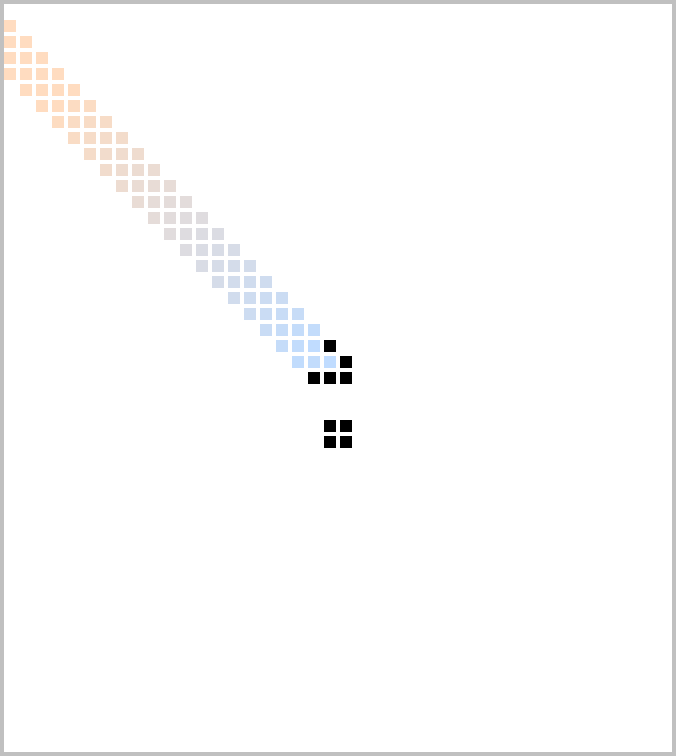
\includegraphics[width=0.3\textwidth]{universal_construction/0degree_hand.png}} \vcenteredhbox{\begin{tabular}{@{}c@{}}\color{black}{$\xrightarrow{\text{\clock{3}{35} 1868}}$} \\ \gliderarrow{19}\end{tabular}} \vcenteredhbox{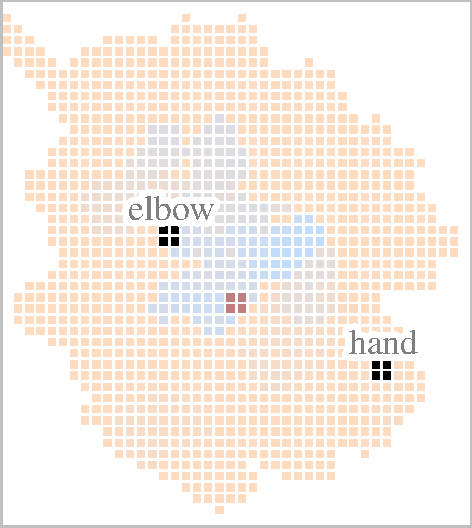
\includegraphics[width=0.3\textwidth]{universal_construction/0degree_hand_2.pdf}}}
	\caption{A single-lane sequence of $19$ gliders creating a hand block for a zero-degree elbow.}\label{fig:0degree_hand}
\end{figure}

Since the hand that this glider sequence creates is fairly close to the zero-degree elbow, it is often a good idea to separate them a bit more by applying one of the elbow-pulling sequences that we have seen. We can use the $12$hd pull from Figure~\ref{fig:0_degree_block_pull}, for example, repeatedly to create as large of a gap between the elbow and hand as we want.

With the glider sequences that we have now seen, it is straightforward to use a zero-degree elbow to synthesize any object that has a slow salvo synthesis no wider than $200$ or so lanes.\footnote{It is actually possible to use a zero-degree elbow to implement \emph{any} slow salvo synthesis (i.e., zero-degree elbows are universal, just like we saw $90$-degree elbows are universal in Theorem~\ref{thm:single_channel_90_degree}). Indeed, we could use the zero-degree elbow to fire a slow salvo that duplicates the hand block, thus leaving us with \emph{three} blocks: the zero-degree elbow block, which fires at a (slow, not single-lane) $90$-degree elbow block, which fires at a target block. However, actually synthesizing anything in this manner is excruciatingly slow, so we do not make use of this technique.} For example, we implement the $4$-glider $(11,0)$ block pull\index{(11,0) block pull} from Figure~\ref{fig:block_move_11_0} via a zero-degree elbow much like we did for the $90$-degree elbow. However, the details work out more simply since we do not have to worry about moving the elbow to a precise location after each slow glider is produced:\smallskip

\begin{itemize}
	\item We first use the hand-making sequence of gliders from Figure~\ref{fig:0degree_hand}. We then want to fire gliders on lanes~$-1$, $-1$, $11$, and $5$, in that order.\smallskip
	
	\item To fire a glider on lane~$-1$, we simply use the appropriate glider sequence from Table~\ref{tab:single_lane_0deg_glider_timings}.\smallskip
	
	\item To fire another glider on lane~$-1$, we have to instead use the glider sequence corresponding to lane~$1$ (since the zero-degree elbow was moved to the other side of the glider sequence in the previous step, which has an odd ``move'' value of $-9$). However, before we can fire this glider, we have to pull the elbow block away from the hand block, or else they would collide with each other at this point. We thus apply the $12$hd pull sequence from Figure~\ref{fig:0_degree_block_pull} twice.\smallskip
	
	\item To fire the third glider on lane $11$, we use the glider sequence corresponding to lane $-11$ (since the elbow block is still on the side of the glider sequence opposite from where it started).\smallskip
	
	\item Since the lane~$-11$ sequence pulled the elbow block by $53$ half-diagonals (which is odd), the zero-degree elbow has now been flipped back to its original side of the glider sequence. We can thus simply use the glider sequence corresponding to lane~$5$ at this point.\smallskip
\end{itemize}

When we put all of this together, we get the following single-lane sequence of $118$ gliders (which we illustrate in Figure~\ref{fig:0_degree_block_move} and specify by $117$ timings between those gliders) that first creates a hand block and then moves that hand block $11$~cells via a sequence of $4$ parallel slow gliders:
\begin{align*}
	& \text{\texttt{\footnotesize make hand: {\footnotesize 109, 90, 93, 91, 91, 90, 90, 100, 90, 90, 146, 96, 90, 90, 90, 92, 156, 144, 90,}}} \\
	& \text{\texttt{\footnotesize ~fire~~-1: {\footnotesize 109, 90, 95, 245, 90, 95, 90, 123, 91, 90, 115, 142, 90,}}} \\
	& \text{\texttt{\footnotesize ~move~-12: {\footnotesize 109, 91, 93, 91, 137, 91, 91, 125, 172, 108, 90, 109, 91, 101, 120, 90, 90,}}} \\
	& \text{\texttt{\footnotesize ~move~-12: {\footnotesize 109, 91, 93, 91, 137, 91, 91, 125, 172, 108, 90, 109, 91, 101, 120, 90, 90,}}} \\
	& \text{\texttt{\footnotesize ~fire~~~1: {\footnotesize 109, 91, 94, 91, 91, 93, 90, 95, 90, 113, 90, 99, 90, 156, 90, 90, 90, 138, 170,}}} \\
	& \text{\texttt{\footnotesize ~fire~-11: {\footnotesize 93, 91, 151, 90, 139, 180, 103, 115, 167, 91, 120, 139, 135, 91, 91, 169,}}} \\
	& \text{\texttt{\footnotesize ~fire~~~5: {\footnotesize 109, 90, 93, 91, 91, 135, 91, 124, 90, 90, 148, 91, 91, 97, 141, 91.}}}
\end{align*}

\begin{figure}[!htb]
	\centering
	\embedlink{0_degree_block_move}{\vcenteredhbox{\phantom{$\cdots$ $\xrightarrow{\text{\clock{2}{12} 1904}}$}} \vcenteredhbox{\patternimg{0.069}{0_degree_block_move_0}} \vcenteredhbox{\begin{tabular}{@{}c@{}}\color{black}{$\xrightarrow{\text{\clock{7}{1} 1904}}$} \\ \gliderarrow{19}\end{tabular}} \vcenteredhbox{\patternimg{0.069}{0_degree_block_move_1}} \vcenteredhbox{\begin{tabular}{@{}c@{}}\color{black}{$\xrightarrow{\text{\clock{11}{20} 1447}}$} \\ \gliderarrow{13}\end{tabular}} \vcenteredhbox{\patternimg{0.069}{0_degree_block_move_2}}} \\[1em]
	
	\patternlink{90_degree_block_move}{\vcenteredhbox{\begin{tabular}{@{}c@{}}\color{black}{$\cdots$ $\xrightarrow{\text{\clock{2}{12} 1775}}$} \\ \hphantom{$\cdots$} \gliderarrow{17}\end{tabular}} \vcenteredhbox{\patternimg{0.069}{0_degree_block_move_3}} \vcenteredhbox{\begin{tabular}{@{}c@{}}\color{black}{$\xrightarrow{\text{\clock{2}{12} 1775}}$} \\ \gliderarrow{17}\end{tabular}} \vcenteredhbox{\patternimg{0.069}{0_degree_block_move_4}} \vcenteredhbox{\begin{tabular}{@{}c@{}}\color{black}{$\xrightarrow{\text{\clock{9}{25} 1923}}$} \\ \gliderarrow{19}\end{tabular}} \vcenteredhbox{\patternimg{0.069}{0_degree_block_move_5}}} \\[1em]
	
	\patternlink{90_degree_block_move}{\vcenteredhbox{\begin{tabular}{@{}c@{}}\color{black}{$\cdots$ $\xrightarrow{\text{\clock{8}{5} 1858}}$} \\ \hphantom{$\cdots$} \gliderarrow{16}\end{tabular}} \vcenteredhbox{\patternimg{0.069}{0_degree_block_move_6}} \vcenteredhbox{\begin{tabular}{@{}c@{}}\color{black}{$\xrightarrow{\text{\clock{9}{25} 1664}}$} \\ \gliderarrow{17}\end{tabular}} \vcenteredhbox{\patternimg{0.069}{0_degree_block_move_8}} \vcenteredhbox{\phantom{\color{black}{\hspace{0.08cm}$\xrightarrow{\text{\clock{6}{45} 138}}$\hspace{0.08cm}}}} \vcenteredhbox{\phantom{\patternimg{0.069}{0_degree_block_move_8}}}}
	
	\caption{A single-lane sequence of 118 gliders creating a hand block and then firing 4 parallel slow gliders at that hand block so as to move it up by 11~cells. The parallel slow gliders are created on the correct lanes by using the sequences from Table~\ref{tab:single_lane_0deg_glider_timings}.}\label{fig:0_degree_block_move}
\end{figure}


%%%%%%%%%%%%%%%%%%%%%%%%%%%%%%%%
\section{Duplicating and Reflecting Single-Channel Recipes}\label{sec:snarkmaker}
%%%%%%%%%%%%%%%%%%%%%%%%%%%%%%%%

Now that we know how to build things with single-channel glider recipes, we would like to be able to manipulate them. In particular, it is going to be important that we are able to reflect these recipes and also duplicate them, so that we can use one copy of the recipe to build something while potentially saving the other copy for later use.

Thanks to the fact that these recipes are single-channel, a single Snark can be used to reflect the entire recipe. However, if there is not already a Snark at the location we would like the reflection to take place, we have to be a bit more clever. In this situation, we can use a single-channel recipe to build a Snark directly in the path of the recipe itself, then let an arbitrary number of gliders be reflected by the Snark, and then use another single-channel recipe to destroy the Snark once it is done being useful. The recipes that create and destroy this in-lane Snark are appropriately called the \emph{Snarkmaker} and \emph{Snarkbreaker}.


%%%%%%%%%%%%%%%%%%%%%%%%%%%%%%%%
\subsection{The Snarkmaker}\label{sec:snarkmaker_itself}\index{Snarkmaker}
%%%%%%%%%%%%%%%%%%%%%%%%%%%%%%%%

The Snarkmaker can be constructed by first searching for a unidirectional slow-salvo recipe for a Snark, and then using the zero-degree elbow toolkit from the previous section to turn it into a single-lane recipe (at the expense of having many more gliders). One unidirectional slow salvo synthesis of a Snark that works is the $95$-glider monstrosity displayed in Figure~\ref{fig:snark_slow_salvo}.\footnote{This salvo was found by Adam P.~Goucher in March 2017.}

\begin{figure}[!htb]
	\centering
	\embedlink{snark_slow_salvo}{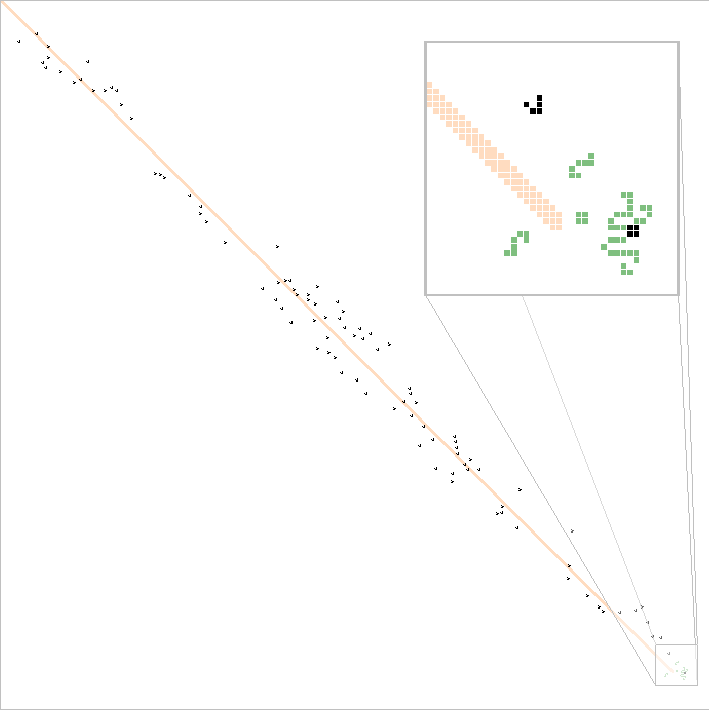
\includegraphics[width=\textwidth]{universal_construction/snark_slow_salvo.pdf}}
	\caption{A $95$-glider unidirectional p$2$ slow salvo synthesis of a Snark. The location of the to-be-constructed Snark is highlighted in \bgbox{greenpastel}{green}, and the lane that it can reflect gliders from is highlighted in \bgbox{orangeback2}{orange}.}\label{fig:snark_slow_salvo}
\end{figure}

We can turn this unidirectional slow salvo into a single-channel recipe by consulting a database of zero-degree single-channel glider sequences. For example, the first glider in the Snark-creating slow salvo is on lane~$15$ (relative to the input lane of the Snark), so it can be created by the lane~$15$ recipe from Table~\ref{tab:single_lane_0deg_glider_timings}:
\begin{center}
	\texttt{\small 109, 90, 93, 91, 91, 158, 94, 113, 91, 90, 91, 96, 90, 142, {\color{gray}(90)}}.
\end{center}
The next glider is on lane~22, so we can again simply use the corresponding recipe from Table~\ref{tab:single_lane_0deg_glider_timings}:
\begin{center}
	\texttt{\small 109, 91, 94, 91, 91, 93, 90, 91, 91, 90, \\ 100, 90, 94, 90, 108, 90, 91, 91, 119, {\color{gray}(90)}}.
\end{center}

After stringing together 95 recipes of this type (one for each glider in the slow salvo),\footnote{This process is completely mechanical, but also extremely tedious, which means it is best done by a computer instead of a human. Also, the particular recipes that we used in the Snarkmaker do not always match up exactly with the recipes from Table~\ref{tab:single_lane_0deg_glider_timings}---multiple recipes are known for most lane numbers.} we get a single-channel recipe consisting of 2,253 gliders that creates a Snark. However, there are still a few other zero-degree elbow recipes that we must prepend and append to make this Snarkmaker actually usable:\smallskip

\begin{itemize}
	\item We first need to use a recipe that creates a block that is offset far to the side, so that the glider recipes that are reflected through the Snark have something to hit (i.e., we need to create a block that will become the 0-degree elbow after the Snark has been made). The 90-degree hand recipe~\eqref{eq:make_hand_90_deg} can carry out this task.\smallskip
	
	\item We then need to use a recipe that creates the zero-degree hand that will be used as the seed for the synthesis of the Snark (i.e., the seed block in Figure~\ref{fig:snark_slow_salvo}). The recipe from Section~\ref{sec:single_channel_zero_make_hand} can carry out this task.\smallskip
	
	\item We need a recipe that can destroy the original zero-degree elbow, since it serves no purpose after the Snark is constructed (and in fact just prevents gliders from entering the Snark). The following 8-glider recipe takes care of this task:
	
	\begin{center}
		\texttt{\small 109, 91, 95, 113, 90, 134, 90, {\color{gray}(90)}}.
	\end{center}
	
	\item Finally, we can use the elbow-moving recipes of Table~\ref{fig:90_degree_block_move} to adjust the relative positioning of the three different elbows that are used throughout all of these operations.\smallskip
\end{itemize}

After we put all of this together, we get a single-channel glider recipe containing a grand total of 2,427 gliders that creates a Snark, and also moves the elbow to its far side so that subsequent glider recipes on that lane hit the elbow after passing through the Snark. This \emph{Snarkmaker} is displayed in Figure~\ref{fig:snarkmaker}, and the complete sequence of glider timings that make it up is provided in Appendix~\ref{sec:appendix_snarkmaker}.

\begin{figure}[!htb]
	\centering
	\embedlink{snarkmaker}{\vcenteredhbox{\patternimg{0.08}{snarkmaker_0}} \vcenteredhbox{\gliderarrow{56}} \vcenteredhbox{\patternimg{0.08}{snarkmaker_56}} \vcenteredhbox{\gliderarrow{34}} \vcenteredhbox{\patternimg{0.08}{snarkmaker_90}} \\[1em] \vcenteredhbox{\phantom{\patternimg{0.075}{snarkmaker_0}}} \vcenteredhbox{\gliderarrow{2253}} \vcenteredhbox{\patternimg{0.08}{snarkmaker_2343}} \,\! \vcenteredhbox{\gliderarrow{8}} \,\! \vcenteredhbox{\patternimg{0.08}{snarkmaker_2351}}}
	
	\caption{The Snarkmaker, which is a single-channel glider recipe that first creates the post-Snark elbow block, then creates a zero-degree elbow, then creates a Snark via that zero-degree elbow, and then finally destroys the zero-degree elbow. Not displayed are 76 (optional) final gliders that are typically appended at the end to push the post-Snark elbow far enough away from the Snark that another Snarkmaker recipe could be used.}\label{fig:snarkmaker}
\end{figure}

Single-channel recipes are also known for creating a Snark in its three other possible orientations.\footnote{These recipes were all found by Adam P.~Goucher in March 2017---see \httpsurl{conwaylife.com/forums/viewtopic.php?f=2\&t=2660\&start=25\#p42121}.} However, they are all roughly as large as the Snarkmaker, and the details of their construction are all very similar to that of the Snarkmaker, so we do not present them here.


%%%%%%%%%%%%%%%%%%%%%%%%%%%%%%%%
\subsection{The Snarkbreaker}\label{sec:snarkbreaker}\index{Snarkbreaker}
%%%%%%%%%%%%%%%%%%%%%%%%%%%%%%%%

The Snarkbreaker is \emph{considerably} simpler than the Snarkmaker.\footnote{In Life, just like in life, it is typically much easier to break something than it is to make it.} Basically all we need is a way of colliding a glider (or gliders) with the Snark so as to destroy it, and a single-channel recipe that creates those gliders. Two reactions that take care of these tasks are displayed in Figure~??.

% FIGURES

The Snarkbreaker is simply the combination of these two reactions, which consists of ?? gliders and the following ?? timings:
\begin{align*}
	& \text{\texttt{\footnotesize return glider: {\footnotesize 93, 91, 118, 93, 151, 90, 99, 155, 120, 92, 108, 90, 102, 164, 90, 90,}}} \\
	& \text{\texttt{\footnotesize Snark destroy: {\footnotesize varies, 143, 97, {\color{gray}(90)}.}}}
\end{align*}

% Talk about "varies" because it depends on how far away the elbow block is



%%%%%%%%%%%%%%%%%%%%%%%%%%%%%%%%
\subsection{The Scorbie Splitter}\label{sec:scorbie_splitter}
%%%%%%%%%%%%%%%%%%%%%%%%%%%%%%%%

Stuff.

% Slow-salvo Snark and other goodies:
%https://conwaylife.com/forums/viewtopic.php?f=2&t=2660&start=25
%x = 641, y = 615, rule = LifeHistory
%639.2E$627.2D10.2E$626.3D$625.4D$624.4D$623.4D$622.4D$621.4D$620.4D$
%619.4D11.2A$618.4D11.A.A$617.4D14.A$616.4D$615.4D$614.4D$613.4D$612.
%4D$611.4D$610.4D$609.4D$608.4D$607.4D$606.4D$605.4D$604.4D18.2A$603.
%4D11.2A5.A.A$602.4D11.A.A7.A$602.3D14.A12$613.2A$612.A.A$614.A8$586.
%2A$569.2A14.A.A$570.2A15.A13.2A$569.A30.A.A$602.A$565.2A40.2A$566.2A
%40.2A$565.A41.A9$554.2A$555.2A$554.A15$535.2A$536.2A$535.A10$536.2A$
%537.2A$536.A32$539.2A$540.2A$539.A$486.2A$485.A.A$487.A12$466.2A$467.
%2A2.2A$466.A3.A.A$472.A4$471.2A$472.2A$471.A14$488.2A$489.2A$488.A6$
%422.2A$423.2A$422.A6$423.2A$422.A.A$424.A2$438.2A9.2A$407.2A28.A.A8.A
%.A$406.A.A30.A10.A$408.A2$435.2A$434.A.A$436.A3$440.2A$441.2A$440.A3$
%428.2A$427.A.A$429.A4$427.2A$426.A.A$391.2A35.A$390.A.A$392.A2$426.2A
%$425.A.A$404.2A21.A$403.A.A$405.A$425.2A$424.A.A$426.A8$395.2A$394.A.
%A$396.A8$383.2A$382.A.A$384.A5$366.2A$367.2A$366.A4$387.2A$376.2A10.
%2A$375.A.A9.A$377.A6$339.2A41.2A$338.A.A40.A.A$340.A42.A3$381.2A$380.
%A.A$382.A6$330.2A$329.A.A$331.A5$315.2A$314.A.A$316.A13$308.2A$309.2A
%$308.A3$302.2A$303.2A$302.A$350.2A$291.2A56.A.A$292.2A57.A$291.A2$
%361.2A$362.2A$361.A3$336.2A$301.2A32.A.A$302.2A33.A$301.A25.2A$328.2A
%$327.A15.2A$342.A.A$344.A3$333.2A$318.2A12.A.A$317.A.A14.A$319.A3$
%266.2A$265.A.A$267.A20.2A$289.2A$288.A24.2A$299.2A11.A.A$300.2A12.A$
%299.A4$316.2A$317.2A$316.A$257.2A$256.A.A$258.A2$289.2A$290.2A$289.A
%21.2A$310.A.A$251.2A29.2A28.A$250.A.A30.2A$252.A29.A3$271.2A9.2A$272.
%2A9.2A$271.A10.A3$268.2A$238.2A29.2A$237.A.A28.A$239.A51.2A$292.2A$
%291.A2$253.2A$254.2A$253.A6.2A3.2A$261.2A.A.A$260.A5.A31$252.2A$253.
%2A$252.A2$201.2A$202.2A$201.A18$183.2A$184.2A$183.A6$177.2A$178.2A$
%177.A5$178.2A$177.A.A$179.A9$167.2A$166.A.A$168.A15$142.2A$143.2A$
%142.A$138.2A$133.2A4.2A$134.2A2.A$133.A52$110.2A$111.2A$110.A11$100.
%2A$101.2A$100.A12$73.2A9.2A10.2A$74.2A9.2A8.A.A$73.A10.A12.A$91.2A$
%90.A.A$92.A3$54.2A$55.2A$54.A$61.2A$60.A.A$62.A5$41.2A$42.2A$41.A2$
%27.2A$26.A.A$28.A3$24.2A$23.A.A42.2A$25.A41.A.A$69.A2$29.2A$30.2A$29.
%A9$29.2A$30.2A$29.A3$.2A$A.A$2.A5$18.2A$17.A.A$19.A!


% TODO: Need scorbie splitter. Maybe a section titled "duplicating a single-channel recipe" or some such? Then give single-channel recipe for it, then an example where it duplicates itself?
%x = 71, y = 68, rule = B3/S23
%9bo$9b3o$12bo$11bobo$11bobo$12bo5$27b2o$27b2o4$7b2o$6bobo$6bo$5b2o7b2o
%$14b2o2$22b2obo$22b2ob3o$28bo$22b2ob3o$23bobo$23bobo$24bo2$25bo$23b3o$
%22bo$22b2o$14b2o$14b2o6$3b2o$4bo$4bobo$5b2o3$2o$bo$bobo$2b2o5$23b2o$
%23bo34bobobobobo$24b3o$26bo31bobo2$58bo3bo2$58bo5bo2$58bo7bo2$68bo2$
%70bo!


%%%%%%%%%%%%%%%%%%%%%%%%%%%%%%%%
\section{A Slow Demonoid}\label{sec:demonoid}
%%%%%%%%%%%%%%%%%%%%%%%%%%%%%%%%

The downside of single-channel glider synthesis versus slow salvo synthesis is that the former requires somewhere around $25$ to $40$ times as many gliders to synthesize the same object (roughly the length of an average elbow-moving sequence followed by a glider-firing sequence). However, the upside of it is that the surrounding circuitry that makes use of the synthesis can be considerably simpler, since it just needs to be able to manipulate gliders along a single lane.

We now demonstrate the utility of single-channel glider synthesis by creating another self-constructing spaceship. This spaceship, which is called a \emph{demonoid}\footnote{The name \emph{demonoid} is a portmanteau of ``diagonal'' and ``Geminoid'', where ``Geminoid'' refers to any Gemini-like spaceship that shuttles one or more construction tapes between two universal constructors.},\index{demonoid}\index{Geminoid} is smaller than the Gemini by roughly one order of magnitude---its bounding box has a side length of approximately $5 \times 10^5$ cells instead of $4 \times 10^6$ cells.
% TODO: Alter footnote here -- Geminoids already discussed earlier
% c/256 = 16384c/4194304

% Give schematic here, or a sequence of schematics.

% There are also Orthogonoid spaceships... (put in footenote? Mention in notes and history?)
%c/256 Demonoid (16384c/4194304):
%* 2-engine and 3-engine Cordership pushes for elbows and target blocks
%* 90-degree elbows for most of the construction
%* Snarkmakers/Snarkbreakers to change the construction arm's direction when needed
%* 135-degree single-channel elbows to shoot down old circuitry (construction arm becomes destruction arm)


% TODO: Circle/highlight/dashed lines around different segments of gliders that do different things?
\begin{figure}[!htbp]
	\centering
	\embedlink{c256_demonoid}{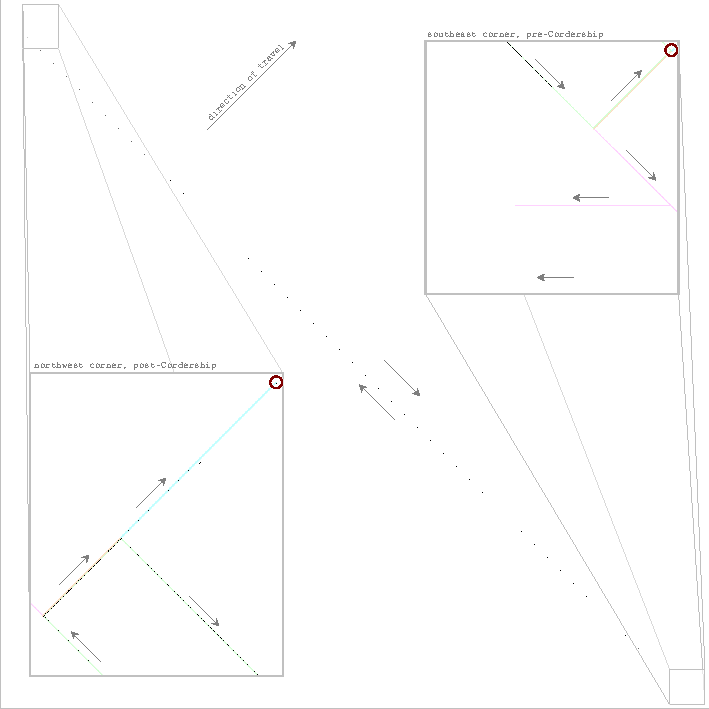
\includegraphics[width=\textwidth]{universal_construction/c256_demonoid.pdf}}
	\caption{A $c/256$ demonoid spaceship that works by bouncing a (very long) single-channel glider recipe (highlighted in \bgbox{greenpastel}{green}) between two self-constructing ends. In the phase shown here, the recipe is about to construct a Cordership in the southeast corner (at the circled location), which moves northeast along the path highlighted in \bgbox{aquaback}{aqua}. The single-channel glider recipe then destroys the Cordership (at the location circled in the northwest corner) so as to leave behind a seed. That seed is then used to build the Snarks and Scorbie splitters necessary to repeat this process. Finally, a single glider is sent backwards to destroy a Snark, letting the single-channel glider recipe follow that path higlighted in \bgbox{magentaback}{magenta}, which is used to destroy old Snarks and Scorbie splitters that are no longer needed.}\label{fig:c256_demonoid}
\end{figure}


%%%%%%%%%%%%%%%%%%%%%%%%%%%%%%%%
\section{A Fast Demonoid}\label{sec:fast_demonoid}
%%%%%%%%%%%%%%%%%%%%%%%%%%%%%%%%

Stuff.


%%%%%%%%%%%%%%%%%%%%%%%%%%%%%%%%
\section{Notes and Historical Remarks}\label{sec:universal_construction_history}
%%%%%%%%%%%%%%%%%%%%%%%%%%%%%%%%

% Maybe note somewhere that pushes tend to be more expensive/rarer than pulls (in all types of circuitry, since the collision starts on the pull side perhaps)

% TAlk about Gemini took 5 months to complete. Maybe earlier instead. Made with a custom computer script to make the glider recipe

The development of single-channel glider synthesis mostly took place in 2017, when a relative newcomer, Simon Ekstr{\"o}m, cavalierly disregarded accumulated prejudices from the previous decade, tried a search, and found that it worked.\footnote{This is not unlike when Andrew J. Wade built Gemini in 2010, or ConwayLife.com forums user ``zdr'' found the copperhead spaceship in 2016. In all of these cases, a newcomer simply looked where the members of the Life community thought there wasn't anything to find.} It was already known in 2015 how to emulate arbitrary glider synthesis via gliders on a single lane, and that technique was used by Chris Cain and Dave Greene to construct an earlier demonoid than the ones we presented in this chapter, called the \emph{0hd demonoid}\index{0hd demonoid} that year.\footnote{The ``0hd'' in the name of this demonoid refers to the fact that there are zero half-diagonals separating its gliders.} However, Ekstr{\"o}m was the first to show that it is possible even when the gliders are far enough apart from each other that they can be fed through components like Snarks and syringes.
% Orthogonoid in the notes/history here?

% TODO: Discuss reverse-caber tosser here, and its ability to construct anything with just a few gliders. This is forward-referenced in Chapter 5.
% Talk about RCT here, and how it shows every glider-synthesizable object can be built wtih 17 far-apart gliders. This is referenced in Ch5 Notes section.


% single channel make xWSS: https://conwaylife.com/forums/viewtopic.php?f=2&t=2660&start=50#p43737
% Exercise: give slow salvo for eater 1 (for example) and ask reader to build it via single-channel 90-degree and then single-channel 0-degree

% exercise with the chirality-swapping 0-degree sequence?
% Exercise based on spiral growth? Or include somewhere? https://www.conwaylife.com/forums/viewtopic.php?f=&p=44792#p44792
% BUILD A GEMINI WITH DIFFERENT PERIOD/SLOPE/WHATEVER
%%%%%%%%%%%%%%%%%%%%%%%%%%%%%%%%%
\section*{Exercises \hfill \normalfont\textsf{\small solutions to starred exercises on \hyperlink{solutions_universal_construction}{page \pageref{solutions_universal_construction}}}}
\label{sec:universal_construction_exercises}
\addcontentsline{toc}{section}{Exercises}
\vspace*{-0.4cm}\hrulefill\vspace*{-0.3cm}\footnotesize\begin{multicols}{2}\vspace*{-0.4cm}\raggedcolumns\interlinepenalty=10000
\setlength{\parskip}{0pt}
%%%%%%%%%%%%%%%%%%%%%%%%%%%%%%%%%


\begin{problem}\label{exer:construction_arm_lanes_timed}
	The elbow-operation circuit of Figure~\ref{fig:construction_arm} requires two synchronized input gliders to trigger each of the \texttt{PUSH}, \texttt{FIRE WHITE}, and \texttt{FIRE BLACK} operations---one to create the frontmost pair of gliders via the \texttt{PULL} circuit, and one to create the additional glider(s).
	
	\noindent Add additional Herschel conduits to that circuit so that each of the four operations can be triggered by just a single input glider.
\end{problem}


\mfilbreak


\begin{problemstar}\label{exer:gemini_unhighlighted_reflectors}
	The two zoom boxes in Figure~\ref{fig:gemini} each have two rows of unhighlighted reflectors that never reflect a single glider. What is their purpose?
\end{problemstar}


\mfilbreak


\begin{problem}\label{exer:block_pull_pond}
	The single-channel elbow-pulling sequence displayed in Figure~\ref{fig:0_degree_block_pull} turns an elbow block into a pond (rather than another block). Why is this not a problem?
\end{problem}
% Pond acts as an elbow in the same way (also explodes into a pi-heptomino)


\mfilbreak


\begin{problemstar}\label{exer:single_lane_glider_final_glider_explain}
	The 185-glider single-lane sequence illustrated in Figure~\ref{fig:90_degree_block_move} makes use of two copies of the glider sequence that moves the elbow forward by $10$ half-diagonals. In the first sequence the final glider arrives after 90~generations, whereas in the second sequence it arrives after 91~generations. Explain the reason for this discrepancy---why can't the final glider in the second sequence also arrive after just 90~generations?
\end{problemstar}


\mfilbreak


\begin{problem}\label{exer:push_elbow_longer}
	The following single-lane glider sequence moves the elbow block:
	\begin{align*}
		& \text{\texttt{\footnotesize~109, 91, 93, 91, 145, 215, 106, 90, 90,}} \\
		& \text{\texttt{\footnotesize~~91, 91, 174, 90, 158, 90, 90, 90, 91,}} \\
		& \text{\texttt{\footnotesize~~~~~~~~~137, 90, 91, 127, {\color{gray}(90)}.}}
	\end{align*}
	
	\begin{enumerate}[label=\bf\color{ocre}(\alph*)]
		\item How many half-diagonals (and in which direction) does this sequence move the elbow?
		% SOLUTION: 20, forward
		
		\item Use this 23-glider sequence to rebuild the 185-glider sequence from Figure~\ref{fig:90_degree_block_move} to be at least $15$~gliders shorter, while still performing the same task (i.e., building a hand block and then moving it south by $11$~cells).
		% SOLUTION: Replace the pair of 10hd moves with this single 20hd move.
	\end{enumerate}
\end{problem}


\mfilbreak


\begin{problemstar}\label{exer:0degree_hand_move}
	What is the ``move'' value of the zero-degree hand-making glider sequence from Figure~\ref{fig:0degree_hand} (i.e., how many half-diagonals is the elbow block moved)?
\end{problemstar}


\mfilbreak


\begin{problem}\label{exer:snark_slow_salvo_pieces}
	The $95$-glider slow salvo synthesis of a Snark from Figure~\ref{fig:snark_slow_salvo} is an incremental synthesis. Break it down into steps like we did with the $94$-glider synthesis from Figure~\ref{fig:17_cell_synthesis}.
\end{problem}

%% EXERCISE END COMMANDS
\end{multicols}
\normalsize\vspace*{0.01cm}
%% DONE EXERCISE END COMMANDS